\documentclass[../labs.tex]{subfiles}

\pagestyle{main}
\renewcommand{\leftmark}{Lab Report \thesection}
\setcounter{section}{2}

\begin{document}




\noindent Steven Labalme\\
TA: Rowan Simonet\\
Lab partners: Eric Yuan and Kate Kaplin\\
12 January 2023\hfill
10 February 2023

\section{UV-VIS ANALYSIS OF IODINE}
\subsection*{Abstract}
% Goals: Experimentally determine several spectroscopic constants of \ce{I2} and use them to calculate the potential energy surface, approximated as a Morse potential, of the ground and second excited states. Compare solution-phase and gas-phase data to obtain insight into how phase changes alter molecular dynamics.
% Results: Calculated the fundamental vibrational frequency, first anharmonicity constant, the well depth, the dissociation energy (from the zero point energy), the difference in energy between the X and B states, and the Morse constant $\beta$.
% Takeaways: Paraphrase from conclusions section.

The goal of this experiment is to determine several spectroscopic constants of iodine and use them to calculate the potential energy surface, approximated as a Morse potential, of the ground and second excited states. Additionally, it is desired to compare solution-phase and gas-phase data to obtain insight into how phase changes alter molecular dynamics.\par
As a result of both gas- and solution-phase analyses, the fundamental vibrational frequency, first anharmonicity constant, well depth, dissociation energy (from the zero point energy), difference in energy between the X and B states, and Morse constant $\beta$ were calculated.\par
The aim is to provide an experimental verification of the basic quantum mechanical theory of molecular transition mechanics.


\subsection*{Introduction}
% Objective.
% Purpose: Experimentally determine several spectroscopic constants of \ce{I2} and use them to calculate the potential energy surface, approximated as a Morse potential, of the ground and second excited states. Data we can obtain: the frequencies and anharmonicities of each electronic state, the dissociation energies of each electronic state\supercite{bib:McNaughtI2}.
% Methods: UV-Vis spectroscopy (gas phase and solution phase), linear regression, theoretical calculations based on the Morse potential. Also McNaught: Care must be taken at the lower ends of $(v',0)$, $(v',1)$, and $(v',2)$, but the hot bands actually make it possible to obtain much more data for our Birge-Sponer plots.
% Background and strategy: The main idea is that incoming radiation couples to the eigenstates of the system. Specifically, frequencies of radiation that (nearly) exactly match the difference in energy between two quantum states are capable of causing a transition. In UV-Vis, this excitation occurs between vibronic energy levels. The electronic energy levels are represented by discrete potential energy surfaces (or wells), and the vibrational energy levels occur as sublevels within the larger electronic levels. If we approximate the electronic potential wells as parabolas (corresponding to a harmonically oscillating molecule), we can prove via quantum mechanics that the energies of the vibrational sublevels depend on an indexing parameter via
% \begin{equation*}
%     E_v = \bar{\nu}_e\left( v+\tfrac{1}{2} \right)
% \end{equation*}
% where $\bar{\nu}_e$ is the fundamental vibrational frequency. Realizing that a harmonic oscillator is not a good approximation, we can introduce anharmonicity into the math by expanding the above energy levels as a power series in $v+1/2$. Using this energy function to second order, we can derive a formula for the spacing between adjacent vibrational energy levels that is linear. Thus, fitting the peaks on a UV-Vis spectrum (which correspond to distinct vibronic transitions) allows us to reverse engineer the fundamental frequency and anharmonicity parameters. These parameters give information on the shape of the potential well that can be fit to a Morse potential. Per \textcite{bib:MorseAccuracy}, the Morse potential is an excellent approximation for the PES of \ce{I2}, even among similar diatomics, so we can expect physically comparable results even from a crude experiment.

% Maybe include $\Delta\nu$, and $\beta$ and $D_e$ equations.
% \emph{cite lab manual.}

The experiment described herein has two main parts. The primary purpose of the first of these is to determine several spectroscopic constants of diatomic iodine (\ce{I2}) from the gas-phase ultraviolet-visible (UV-Vis) absorption spectrum and use them to calculate the potential energy surface, approximated as a Morse potential, of the ground (${}^1\Sigma_\text{g}^+$) and second excited (${}^3\Pi_\text{ou}^+$) states\supercites{bib:LabManual}{bib:McNaughtI2}. The primary purpose of the second of these is obtain a solution-phase UV-Vis absorption spectrum and, from it, calculate the molar extinction coefficient.\par
From the gas-phase data in particular, we can obtain the frequencies, anharmonicities, and magnitudes of each electronic state, the dissociation energies of each electronic state, and more, but we will only focus on the first two herein\supercite{bib:McNaughtI2}. From the solution-phase data, we can only obtain the frequency and magnitude of the transition.\par
As mentioned above, we will collect our data via UV-Vis spectroscopy (gas phase and solution phase). We will analyze anharmonicity (and its derived constants) using a linear model and hence linear regression. All theoretical calculations build up to the construction of a Morse potential.\par
The main theoretical idea behind the experiment is that incoming radiation couples to the eigenstates of the system. Specifically, frequencies of radiation that (nearly) exactly match the difference in energy between two quantum states are capable of causing a transition. In the UV-Vis range, this excitation occurs between vibronic energy levels. The electronic energy levels are represented by discrete potential energy surfaces (PES's), and the vibrational energy levels occur as sublevels within the larger electronic levels. If we approximate the electronic potential wells as parabolas (corresponding to a harmonically oscillating molecule), we can prove via quantum mechanics that the energies of the vibrational sublevels depend on an indexing parameter $v$ via
\begin{equation*}
    E_v = \bar{\nu}_e\left( v+\tfrac{1}{2} \right)
\end{equation*}
where $\bar{\nu}_e$ is the fundamental vibrational frequency. Realizing that a harmonic oscillator is not a good approximation, we can introduce anharmonicity into the math by expanding the above energy levels as a power series in $v+1/2$. Using this energy function to second order, we can derive a formula for the spacing between adjacent vibrational energy levels that is linear. This formula comes in two flavors, one for changes in the vibrational energy level to which an electron is excited and one for changes in the ground state vibrational energy level (i.e., fundamental transitions vs. hot bands). Both are listed below.
\begin{align*}
    \Delta\bar{\nu}(v') &= \bar{\nu}_e'-2\bar{\nu}_e'x_e'(v'+1)&
    \Delta\bar{\nu}(v'') &= \bar{\nu}_e''-2\bar{\nu}_e''x_e''(v''+1)
\end{align*}
In the above equations, $x_e$ is the first anharmonicity constant, and the other variables are as defined above.\par
Thus, fitting the peaks on a UV-Vis spectrum (which correspond to distinct vibronic transitions) allows us to reverse engineer the fundamental frequency and anharmonicity parameters. These parameters give information on the shape of the potential well that can be fit to a Morse potential via\supercite{bib:LabManual}
\begin{align*}
    D_e &\approx \frac{\bar{\nu}_e}{4x_e}&
    \beta &= \bar{\nu}_e\pi\cdot\sqrt{\frac{2c\mu}{hD_e}}
\end{align*}
In the above equations, $c=\SI{2.998e8}{\meter\per\second}$ is the speed of light, $\mu=\SI{1.06e-25}{\kilo\gram}$ is the reduced mass of \ce{I2}, $h=\SI{6.626e-34}{\joule\second}$ is Planck's constant, and all other variables are as defined above.\par
Per \textcite{bib:MorseAccuracy}, the Morse potential is an excellent approximation for the PES of \ce{I2}, even among similar diatomics, so we can expect physically comparable results from the following equation even using such a crude experiment and theoretical model.
\begin{equation*}
    U(r) = D_e(\e[-\beta(r-r_e)]-1)^2
\end{equation*}
In the above equation, $U$ is the potential energy, $r$ is the bond distance on which $U$ depends, $\beta$ is the Morse constant, $r_e$ is the equilibrium constant, and e is Euler's number.


\subsection*{Experimental}
% Note that care must be taken at the lower ends of $(v',0)$, $(v',1)$, and $(v',2)$, but the hot bands actually make it possible to obtain much more data for our Birge-Sponer plots.
% Methods and materials: Ocean Optics USB4000 to collect the spectrum in chloroform. An apparatus the centerpiece of which is an SPEX 500M monochromator, but it also includes a light source, \ce{I2} sample, light shutter, and RCA 6217 photomultiplier tube as a detector. Data collection was performed in LabView from National Instruments.
% Summary of experimental procedures: Do a broad-spectrum scan to identify the region of interest. Do a narrow spectrum, more dense scan to get more precise data. Calibration step (mercury standard of known wavelength; see what's reported as the wavelength and adjust). Then for the solution, take a chloroform and cuvette background, a dark background, and then dilute the sample (expound on this! \SI{0.01}{\molar} stock solution and $\SI{0.7}{\milli\liter}\to\SI{25}{\milli\liter}$ dilution to yield a \SI{2.8e-4}{\molar} solution.) and measure it.
% Safety: Goggles and gloves were used when handling the chloroform-containing samples.

To collect the gas-phase spectrum, an apparatus centered around a SPEX 500M monochromator was used. Said apparatus also included a light source, the \ce{I2} sample, a light shutter, and an RCA 6217 photomultiplier tube (PMT) which functioned as a detector. Removal of external light was accomplished by carrying out the experiment in a darkened room and shrouding the PMT in an additional blanket. Data collection was performed in LabView from National Instruments\supercite{bib:LabManual}. During the post-collection analysis phase, extra care was taken at the lower ends of $(v',0)$, $(v',1)$, and $(v',2)$ peaks since hot bands eventually outweigh other data. However, the hot bands were still analyzed as they actually make it possible to obtain much more data from the excited-state Birge-Sponer plot, and data at all for a ground-state Birge-Sponer plot\supercite{bib:McNaughtI2}.\par
To collect the solution-phase spectrum, an Ocean Optics USB4000 spectrometer was connected to a standard desktop computer running OceanView. The solvent used for \ce{I2} was chloroform (\ce{CHCl3}). An extremely dilute sample was used to bring the data in to the Beer's Law region (to allow for calculation of the molar extinction coefficient, as previously mentioned). Beer's law is given by
\begin{equation*}
    A = \varepsilon bC
\end{equation*}
where $A$ is absorbance, $\varepsilon$ is the molar extinction coefficient, $b$ is the path length (\SI{1}{\centi\meter} in this case since that's the width of the cuvette), and $C$ is the concentration of the dilution (\SI{2.8e-4}{\molar} in this case).\par
The overall procedure was as follows. First, a broad-spectrum scan of the gas-phase sample was collected to identify the region of interest. Next, a narrow-range spectrum was collected to far greater accuracy, allowing for the resolution of vibrational transitions. A subsequent calibration step (using a mercury lamp that emits at one known characteristic wavelength) was performed to account for any error in the monochromator. For the solution, a chloroform and cuvette background, and a dark background were taken. Then, the sample was diluted using \SI{0.7}{\milli\liter} of a \SI{0.01}{\molar} stock solution and an additional \SI{24.3}{\milli\liter} of pure chloroform; the result was a \SI{2.8e-4}{\molar} solution of \ce{I2} in \ce{CHCl3}. Lastly, a UV-Vis absorption spectrum of this sample was taken.\par
Safety goggles and nitrile gloves were used at all times when handling chloroform-containing samples.


\subsection*{Results}
% Logical stepwise presentation of data and relevant analysis, pointing out important milestones and outcomes (including those reported in figures and tables) along the way.
% Specify horizontal/vertical axis in text (e.g., "a plot of y vs. x (Figure ??) reveals that..."). Why are these variables good and how do we know we're measuring them accurately? (Here, we know because we took a baseline with the mercury lamp.)

As determined by the initial broad-spectrum scan, the gas-phase spectrum was collected between \SIrange{5000}{6500}{\angstrom}. It is plotted below in Figure \ref{fig:I2Spectrum3}. Note that the colored numbers correspond to the wavelengths of certain vibrational transitions (green for ground state, orange for the first hot band, red for the second hot band).
\begin{figure}[H]
    \centering
    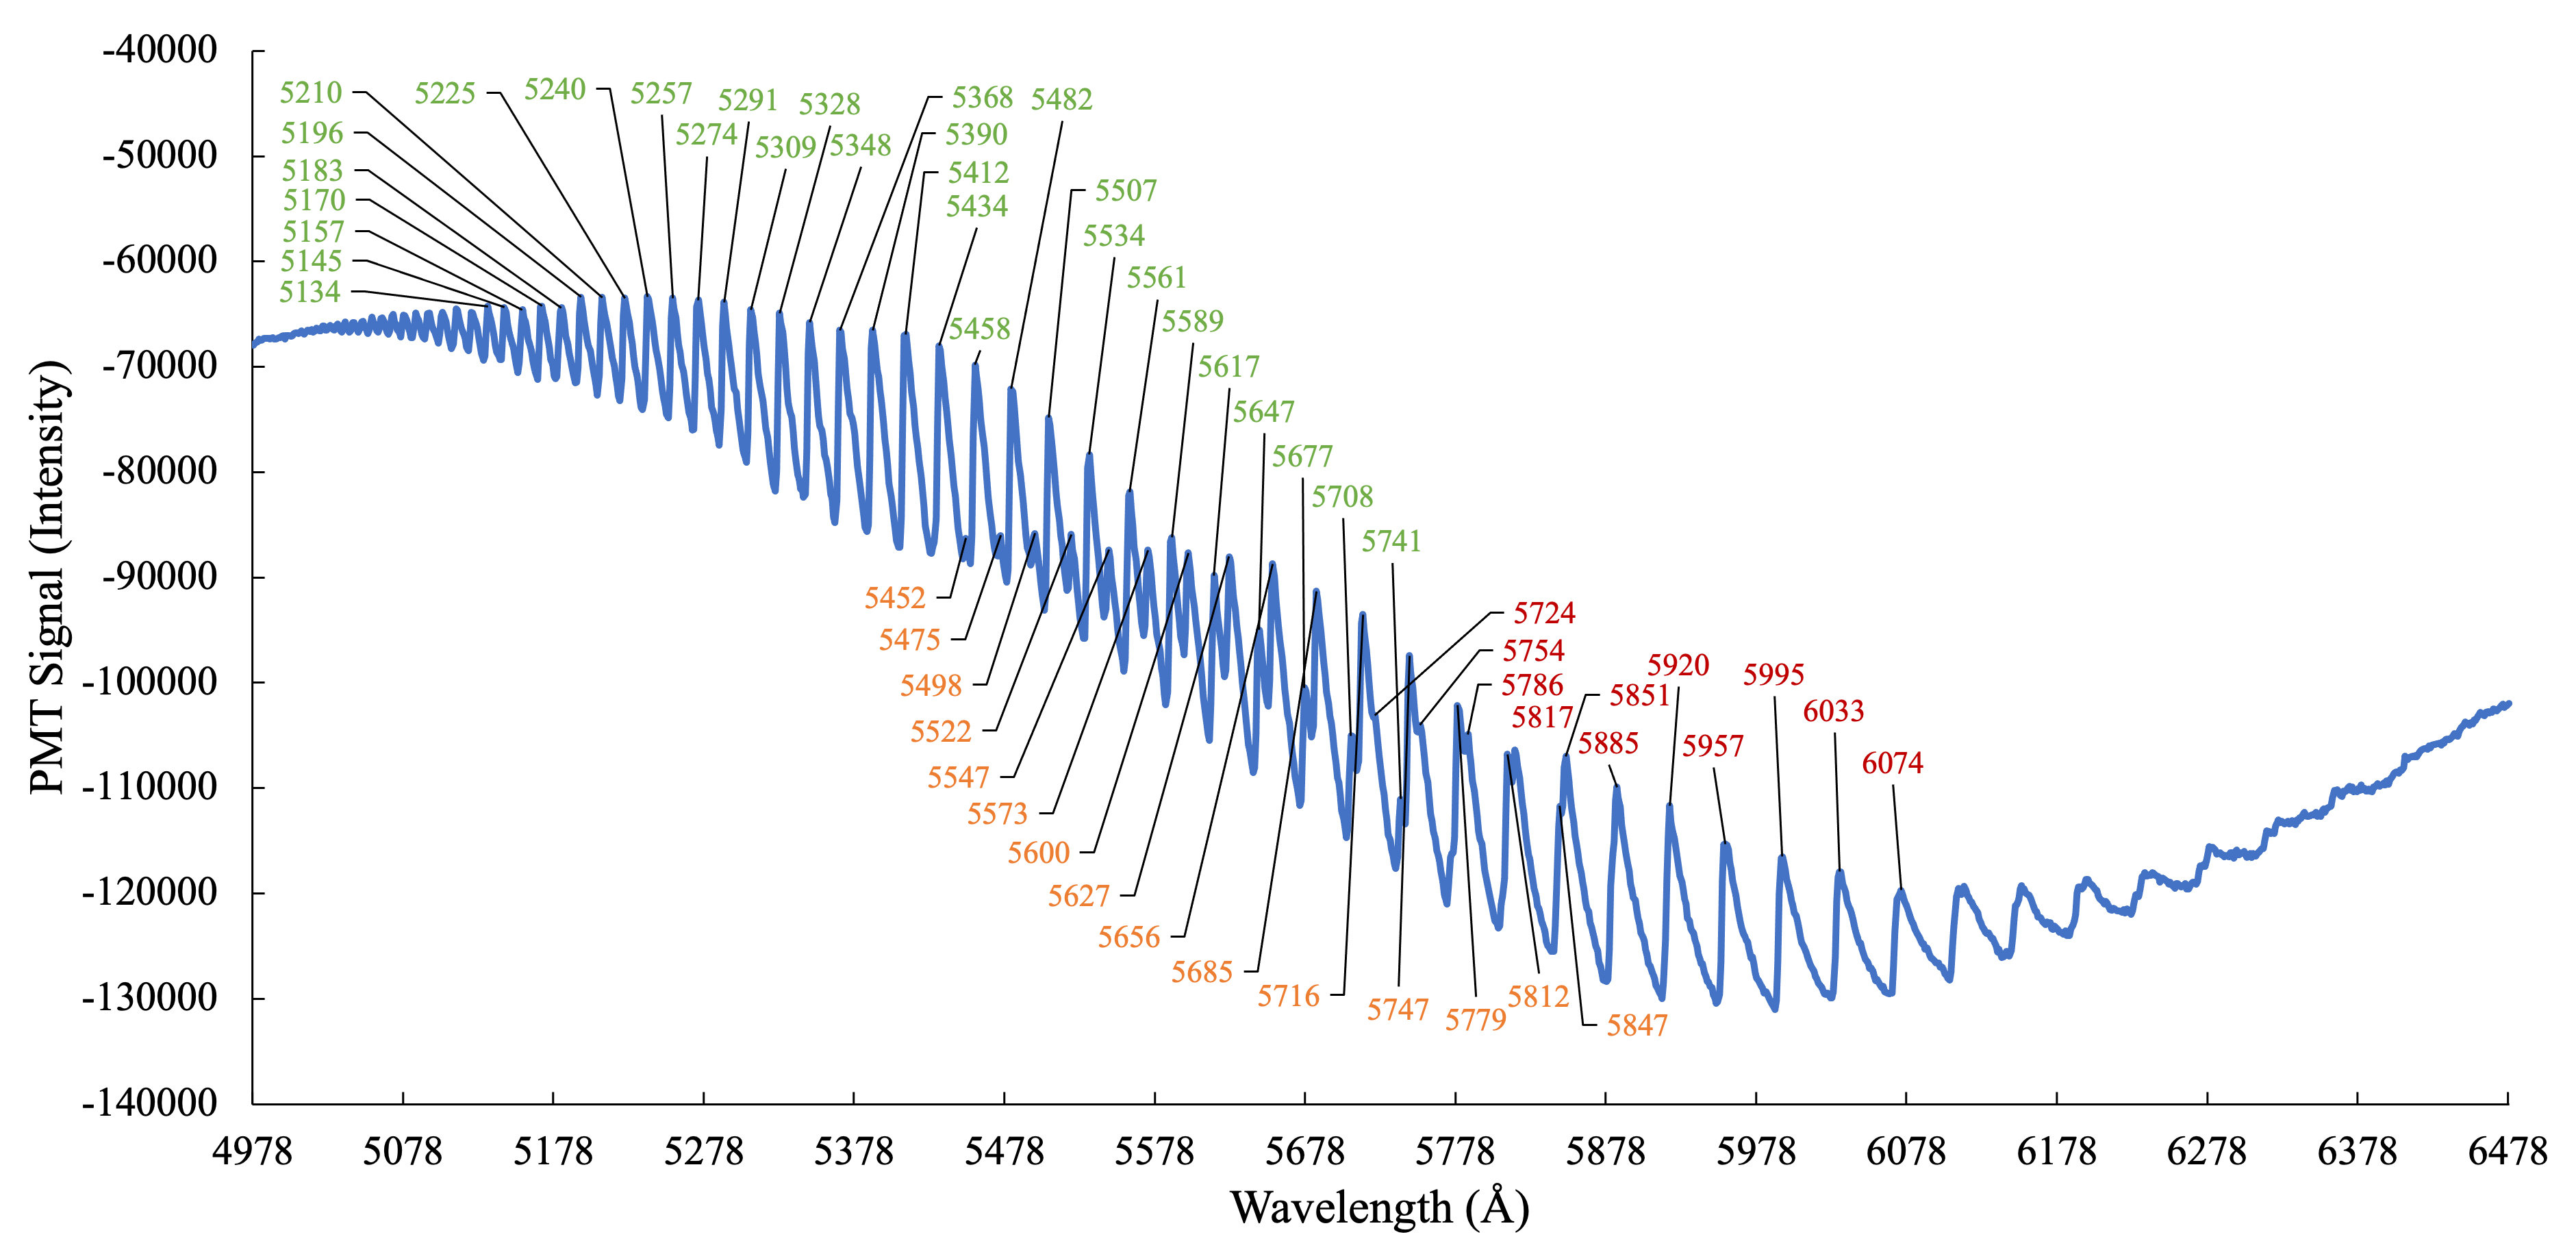
\includegraphics[width=0.95\linewidth]{lab3-I2Spectrum.png}
    \caption{The absorption spectrum of gaseous \ce{I2} between $\lambda=\SIrange{5000}{6500}{\angstrom}$.}
    \label{fig:I2Spectrum3}
\end{figure}
Since the PMT is not capable of measuring absorption directly and unforeseen circumstances prevented the collection of a background spectrum in a timely manner, the spectrum is plotted in \emph{intensity} vs. wavelength instead of the standard \emph{absorption} vs. wavelength. Support for an accurate measurement of the wavelength comes from the aforementioned mercury lamp calibration step, and steps have been taken to ensure that the PMT intensity (as described above) is also accurate.\par
The overall trend observed in Figure \ref{fig:I2Spectrum3} is representative of the electronic absorption band, while the fine structure is vibrational in nature. The variable peak spacing is representative of anharmonicity and is characterized below in Figure \ref{fig:BirgeSponerB3}.\par
First, though, the peaks labeled in Figure \ref{fig:I2Spectrum3} are tabulated and assigned to vibronic transitions using known reference values. The result is as follows. Note that wavelength has been converted to wavenumber.
\begin{table}[H]
    \centering
    \small
    \renewcommand{\arraystretch}{1.2}
    \begin{tabular}{|c|c|c|c|c|c|c|c|c|}
        \hline
        $\bm{v'}$ & $\bm{v''}$ & $\bm{\omega\ (\textbf{cm}^{-1})}$ & $\bm{v'}$ & $\bm{v''}$ & $\bm{\omega\ (\textbf{cm}^{-1})}$ & $\bm{v'}$ & $\bm{v''}$ & $\bm{\omega\ (\textbf{cm}^{-1})}$\\
        \hline
           &   &       &    &   &       & 10 & 2 & 16464\\ \hline
           &   &       &    &   &       & 11 & 2 & 16576\\ \hline
           &   &       &    &   &       & 12 & 2 & 16681\\ \hline
           &   &       &    &   &       & 13 & 2 & 16787\\ \hline
           &   &       & 14 & 1 & 17103 & 14 & 2 & 16892\\ \hline
        15 & 0 & 17419 & 15 & 1 & 17206 & 15 & 2 & 16992\\ \hline
        16 & 0 & 17519 & 16 & 1 & 17304 & 16 & 2 & 17091\\ \hline
        17 & 0 & 17615 & 17 & 1 & 17400 & 17 & 2 & 17191\\ \hline
        18 & 0 & 17709 & 18 & 1 & 17495 & 18 & 2 & 17283\\ \hline
        19 & 0 & 17803 & 19 & 1 & 17590 & 19 & 2 & 17379\\ \hline
        20 & 0 & 17892 & 20 & 1 & 17680 & 20 & 2 & 17470\\ \hline
        21 & 0 & 17982 & 21 & 1 & 17771 &    &   &      \\ \hline
        22 & 0 & 18070 & 22 & 1 & 17857 &    &   &      \\ \hline
        23 & 0 & 18159 & 23 & 1 & 17944 &    &   &      \\ \hline
        24 & 0 & 18242 & 24 & 1 & 18028 &    &   &      \\ \hline
        25 & 0 & 18322 & 25 & 1 & 18109 &    &   &      \\ \hline
        26 & 0 & 18402 & 26 & 1 & 18188 &    &   &      \\ \hline
        27 & 0 & 18477 & 27 & 1 & 18265 &    &   &      \\ \hline
        28 & 0 & 18553 & 28 & 1 & 18342 &    &   &      \\ \hline
        29 & 0 & 18629 &    &   &       &    &   &      \\ \hline
        30 & 0 & 18699 &    &   &       &    &   &      \\ \hline
        31 & 0 & 18769 &    &   &       &    &   &      \\ \hline
        32 & 0 & 18836 &    &   &       &    &   &      \\ \hline
        33 & 0 & 18900 &    &   &       &    &   &      \\ \hline
        34 & 0 & 18961 &    &   &       &    &   &      \\ \hline
        35 & 0 & 19022 &    &   &       &    &   &      \\ \hline
        36 & 0 & 19084 &    &   &       &    &   &      \\ \hline
        37 & 0 & 19139 &    &   &       &    &   &      \\ \hline
        38 & 0 & 19194 &    &   &       &    &   &      \\ \hline
        39 & 0 & 19246 &    &   &       &    &   &      \\ \hline
        40 & 0 & 19294 &    &   &       &    &   &      \\ \hline
        41 & 0 & 19342 &    &   &       &    &   &      \\ \hline
        42 & 0 & 19391 &    &   &       &    &   &      \\ \hline
        43 & 0 & 19436 &    &   &       &    &   &      \\ \hline
        44 & 0 & 19478 &    &   &       &    &   &      \\ \hline
    \end{tabular}
    \caption{Peaks and their corresponding transitions.}
    \label{tab:peakTransition3}
\end{table}
Using the data in Table \ref{tab:peakTransition3} and the $\Delta\bar{\nu}(v')$ equation from the introduction, it is possible to construct and characterize a Birge-Sponer plot (Figure \ref{fig:BirgeSponerB3}) to determine both the fundamental vibration frequency and the first anharmonicity constant. All three data sets ($v''=0,1,2$) are plotted on top of each other, and are plotted versus the change in wavenumber.
\begin{figure}[H]
    \centering
    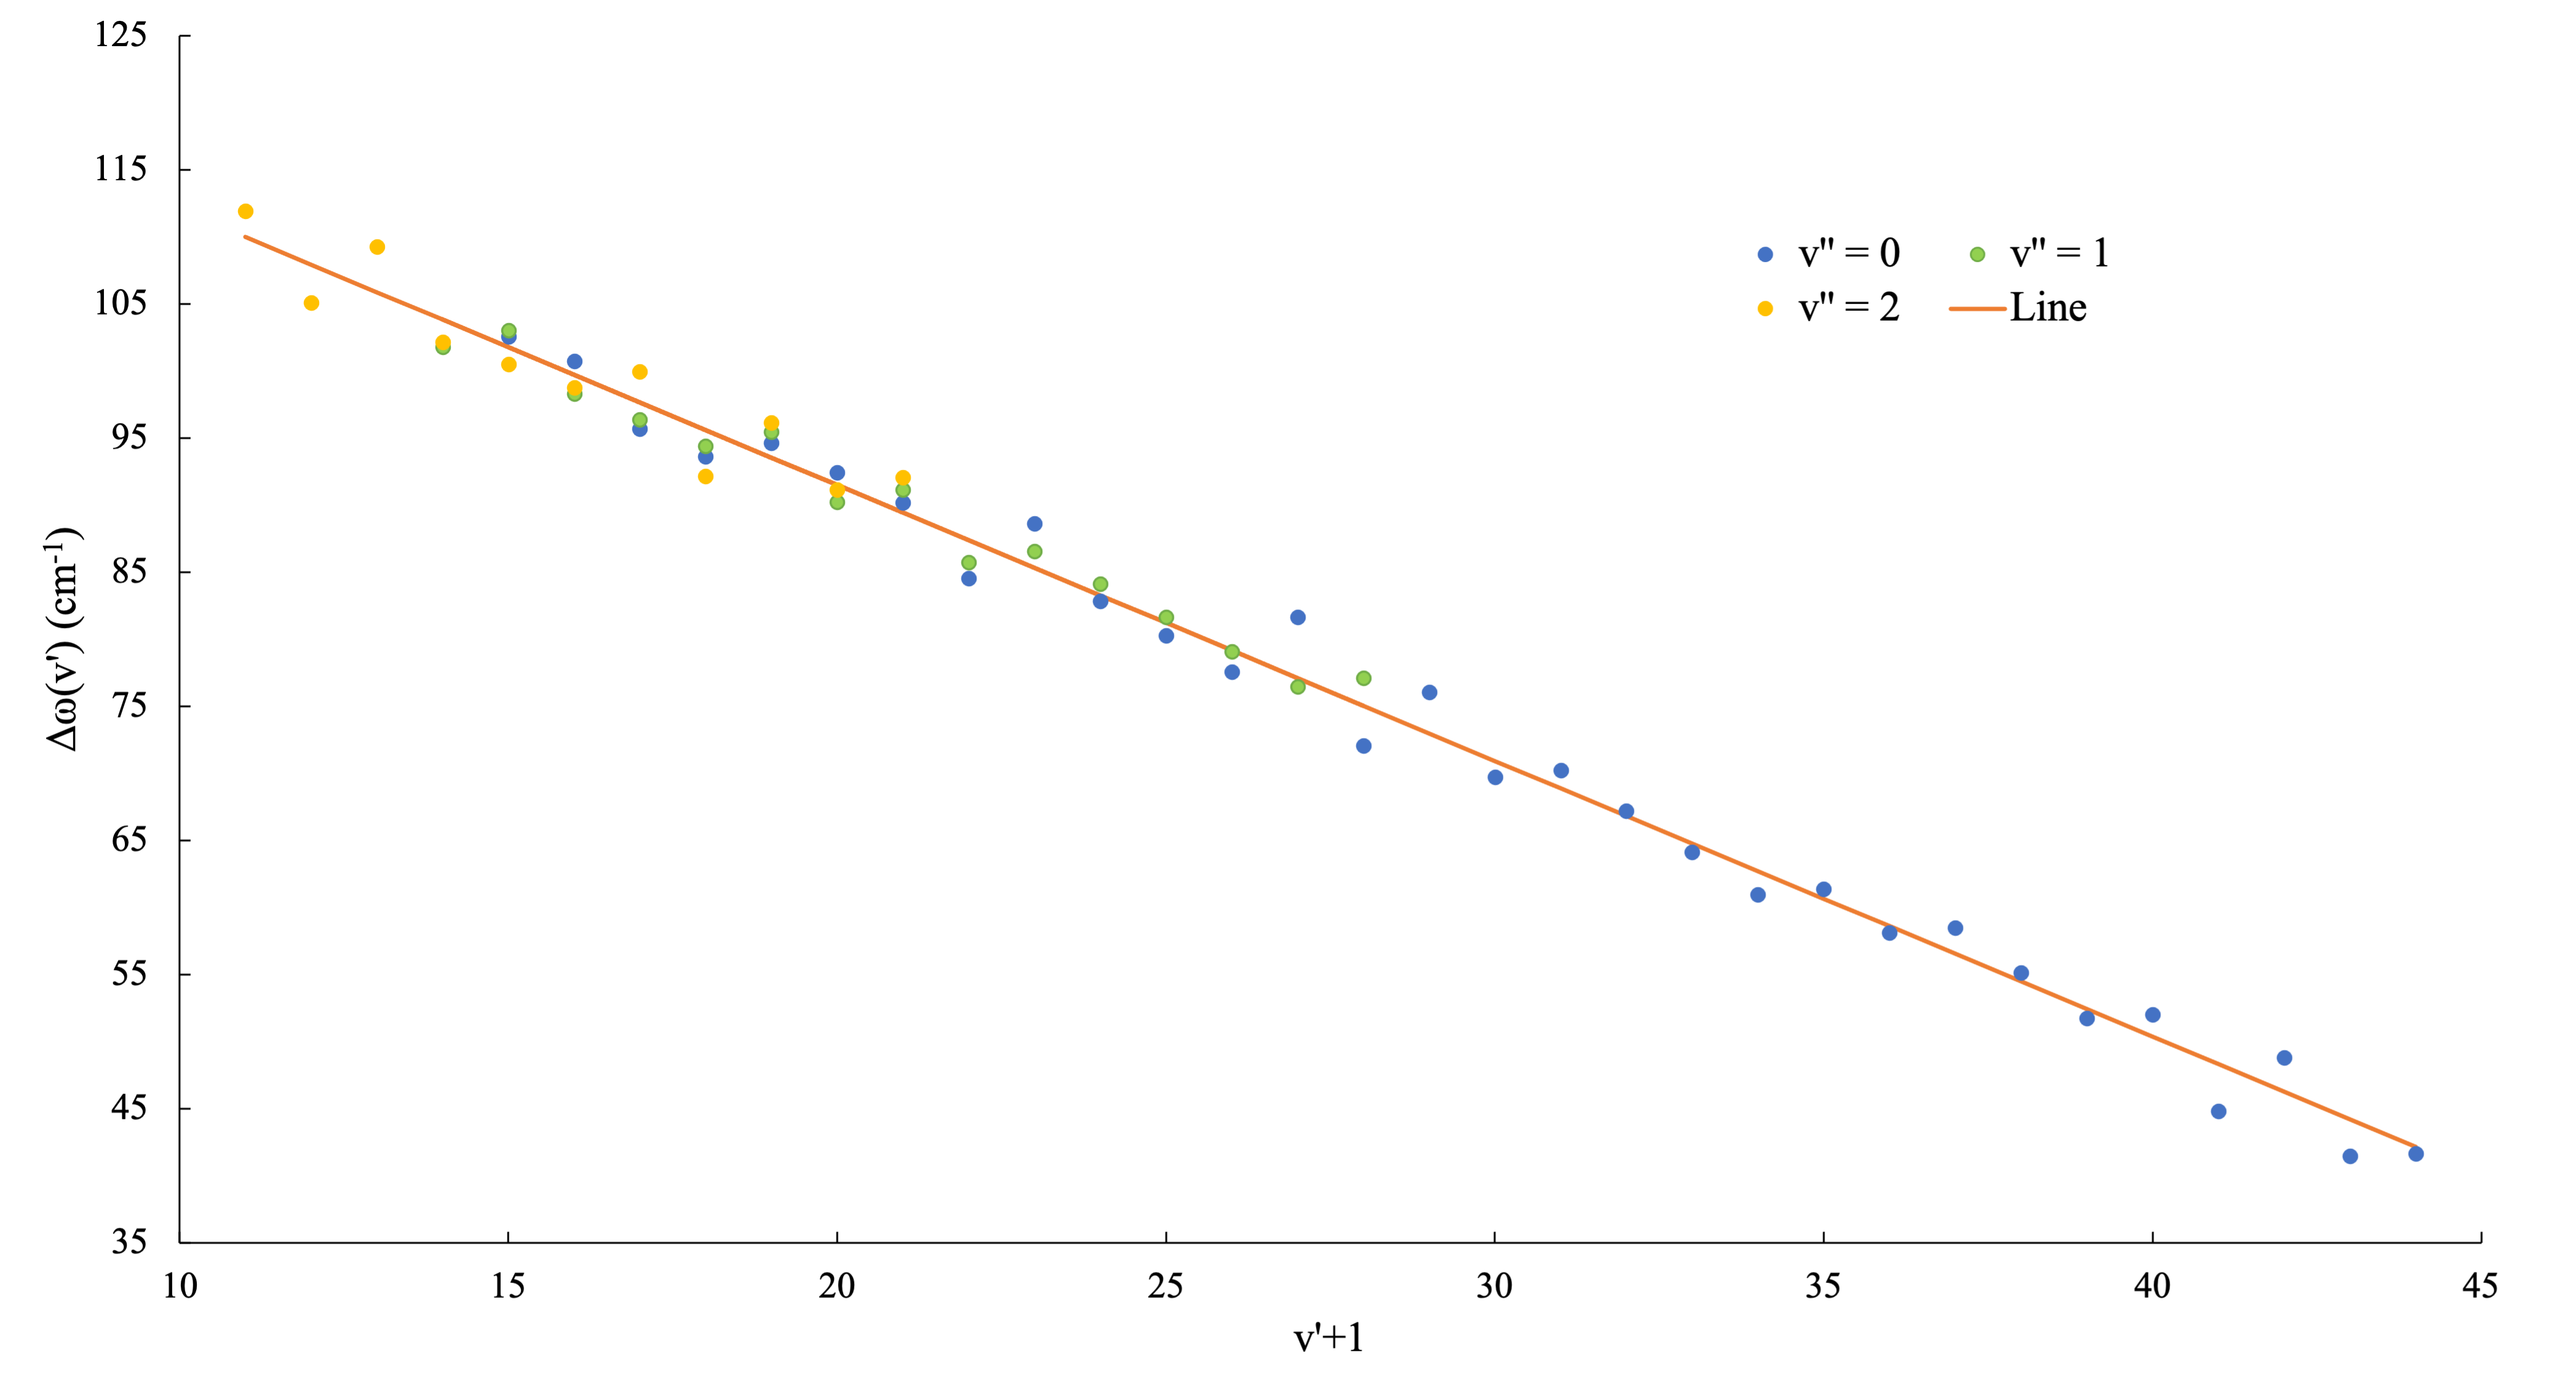
\includegraphics[width=0.95\linewidth]{lab3-BirgeSponerB.png}
    \caption{Birge-Sponer plot for the B state.}
    \label{fig:BirgeSponerB3}
\end{figure}
Evidently, the linear analysis provides a remarkable fit to the data, and it is not immediately obvious that a higher-order energy equation (e.g., cubic, quartic, etc.) would have been necessary to account for additional anharmonicity.\par
The above analysis was repeated for the $\Delta\bar{\nu}(v'')$ data. From $\bar{\nu}_e'$, $\var{\nu}_e'x_e'$, $\bar{\nu}_e''$, and $\var{\nu}_e''x_e''$, the ground and excited state dissociation energies from both the bottom of the energy well and the zero point energy can be calculated: $D_e'$, $D_0'$, $D_e''$, and $D_0''$. The calculation of the energy gap between electronic levels $T_e$ followed from the previous data and additional information on the hypothetical energy of a dissociated excited \ce{I2} molecule. All constants are summarized below.
\begin{table}[H]
    \centering
    \small
    \renewcommand{\arraystretch}{1.2}
    \begin{tabular}{|c|c|c|c|c|c|c|c|c|c|}
        \hline
         & $\bm{\bar{\nu}_e'}$ & $\bm{\bar{\nu}_e'x_e'}$ & $\bm{D_e'}$ & $\bm{D_0'}$ & $\bm{\bar{\nu}_e''}$ & $\bm{\bar{\nu}_e''x_e''}$ & $\bm{D_e''}$ & $\bm{D_0''}$ & $\bm{T_e}$\\
        \hline
        \textbf{Calculated values} & \num{132.22} & \num{1.019} & \num{4288.6} & \num{4222.7} & \num{214.97} & \num{0.912} & \num{12672} & \num{12564} & \num{15986.11}\\
        \hline
        \textbf{Literature values} & \num{125.69}\supercite{bib:NISTDiatomics} & \num{0.764}\supercite{bib:NISTDiatomics} & \num{5169.3} & \num{5106.6} & \num{214.50}\supercite{bib:NISTDiatomics} & \num{0.614}\supercite{bib:NISTDiatomics} & \num{18734} & \num{18627} & \num{15769.01}\supercite{bib:NISTDiatomics}\\
        \hline
    \end{tabular}
    \caption{Calculated spectroscopic constants and their reported values.}
    \label{tab:UVVisConstants3}
\end{table}
Note that the unit for all values in Table \ref{tab:UVVisConstants3} is \si{\per\centi\meter}. Also note that the $D_e$ and $D_0$ values were calculated from the NIST $\bar{\nu}_e'$ and $x_e'=\bar{\nu}_e'x_e'/\bar{\nu}_e'$ values using Equations 9 and 12 in \textcite{bib:LabManual}, respectively.\par
The experimental values in Table \ref{tab:UVVisConstants3} may be plugged into two Morse potential equations as follows. $D_e$ values go in directly. $\beta$ values must be calculated as in the introduction. Equilibrium bond length values are found in \textcite{bib:LabManual}. And $T_e$ gives the vertical offset between the two equations (the zero of energy was arbitrarily defined to be the bottom of the ground (X) state potential well).\par
Additionally, as as wavenumbers have been used throughout the analysis, they are used as the unit of energy on the $y$-axis of Figure \ref{fig:Morse3} below. Lastly, angstroms are a natural scale on which to discuss molecules, so bond length (the $x$-axis below) is given in terms of it. All above determinations of error suggest that the variables are being measured largely accurately.
\begin{figure}[H]
    \centering
    \begin{tikzpicture}[
        xscale=3,yscale=2,
        every node/.style={black}
    ]
        \small
        \draw (2,3) -- node[rotate=90,above=1cm]{Energy (\si{\per\centi\meter})} (2,0) -- node[below=3mm]{Bond length (\si{\angstrom})} (5,0);

        \footnotesize
        \node [below] at (2,0) {2};
        \node [left]  at (2,0) {0};
        \foreach \x in {2.5,...,5} {
            \draw (\x,0.03) -- (\x,0) node[below]{\x};
        }
        \foreach \y/\nam in {0.5/5000,1/10000,1.5/15000,2/20000,2.5/25000,3/30000} {
            \draw (2.03,\y) -- (2,\y) node[left]{\num{\nam}};
        }

        \draw [rex,thick] plot[domain=2.4987:5,variable=\r,smooth,samples=100] (\r,{0.42886*(e^(-1.9650*(\r-3.024))-1)^2+1.5986}) node[above left]{B state};
        \draw [rex,thick] plot[domain=2.165:5,variable=\r,smooth,samples=100] (\r,{1.2672*(e^(-1.8585*(\r-2.666))-1)^2}) node[above left]{X state};
    \end{tikzpicture}
    \caption{Morse potential curves.}
    \label{fig:Morse3}
\end{figure}
From the above plot, it can be seen that the excited state has a slightly longer average bond length (as is to be expected for a molecule that is vibrating more extremely). Additionally, the ground state energies are generally more concentrated in one area, whereas the excited state ones are more spread out.\par
Lastly, all of the gas-phase analysis above is compared to the solution phase data. Both the initial data from Figure \ref{fig:I2Spectrum3} (or rather a separate data set in terms of the molar extinction coefficient, which is closely related to absorption, obtained from \textcite{bib:gasI2}) and the solution-phase data are plotted in Figure \ref{fig:solutionGas3} on the same set of axes. Expressing the data in terms of molar extinction coefficient is driven by the nature of the data from \textcite{bib:gasI2}; data from the solution-phase experiment performed by the authors is readily converted from absorption to molar extinction coefficient using Beer's law (per the introduction). Wavelength has been adjusted for as previously mentioned.
\begin{figure}[H]
    \centering
    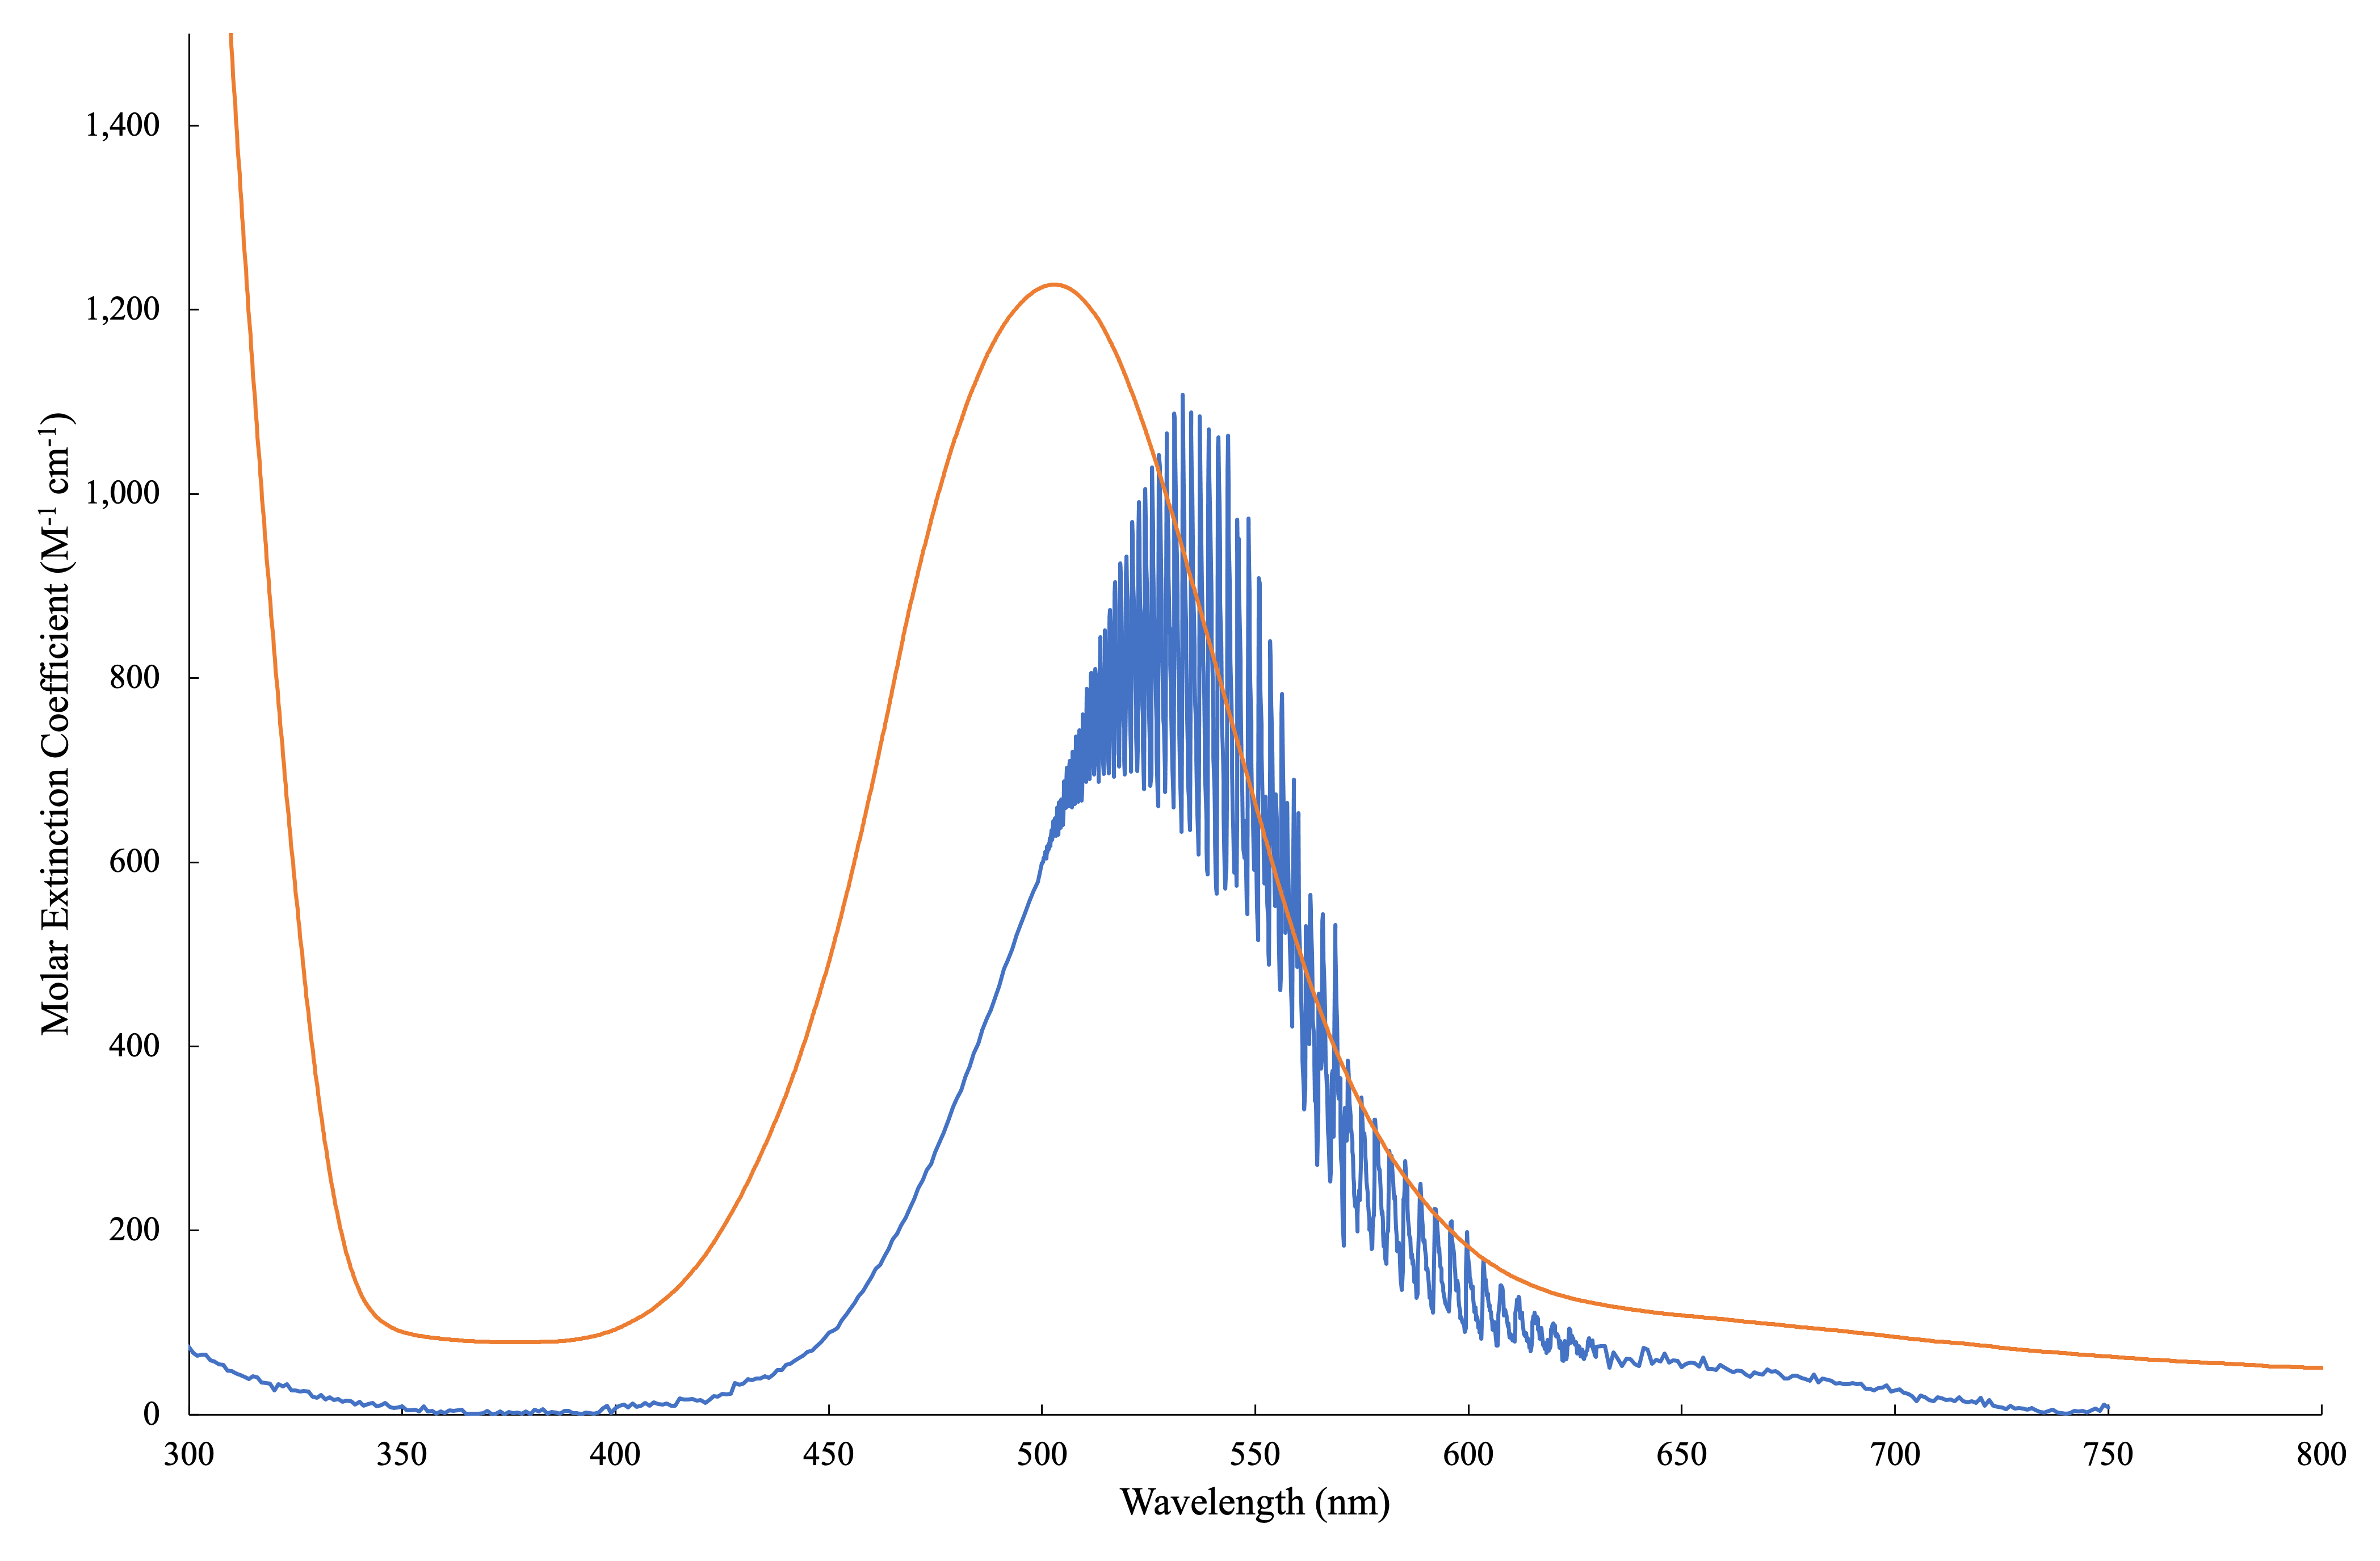
\includegraphics[width=0.95\linewidth]{lab3-solutionGas.png}
    \caption{The absorption spectrum (in terms of the directly proportional molar extinction coefficient) of gaseous\supercite{bib:gasI2} (blue) and chloroform-based (orange) \ce{I2} between $\lambda=\SIrange{300}{800}{\nano\meter}$.}
    \label{fig:solutionGas3}
\end{figure}
The maximum of the gas-phase electronic band is \SI{1089}{\per\molar\per\centi\meter} and occurs at $\lambda=\SI{534.9}{\nano\meter}$. The maximum of the solution-phase electronic band is \SI{1227}{\per\molar\per\centi\meter} at $\lambda=\SI{502.7}{\nano\meter}$.\par
Half the gas-phase electronic maximum is \SI{544.5}{\per\molar\per\centi\meter}. The line $\varepsilon=\SI{544.5}{\per\molar\per\centi\meter}$ intersects the left side of the peak at $\lambda=\SI{496}{\nano\meter}$ and the right side between $\lambda=\SIrange{548.1}{565.8}{\nano\meter}$. Taking the average yields
\begin{equation*}
    \frac{548.1+565.8}{2} = 557.0
\end{equation*}
% with error
% \begin{equation*}
%     \sigma_{\lambda_2} = \sqrt{\frac{(548.1-557.0)^2+(565.8-557.0)^2}{2-1}}
%     = 12.49
% \end{equation*}
Thus, the full width of the absorption band at half the maximum height (FWHM) is
\begin{equation*}
    \text{FWHM} = 557.0-496 = \SI{61}{\nano\meter}
\end{equation*}
% with error
% \begin{equation*}
%     \sigma_\text{FWHM} = \sqrt{\sigma_{\lambda_1}^2+\sigma_{\lambda_2}^2}
%     = \sqrt{1^2+12.49^2}
%     = 12.53
% \end{equation*}\par
Half of the solution-phase electronic maximum is \SI{613.5}{\per\molar\per\centi\meter}. The line $\varepsilon=\SI{613.5}{\per\molar\per\nano\meter}$ intersects the left side of the peak at $\lambda_1=\SI{456.7}{\per\nano\meter}$ and the right side at $\lambda_2=\SI{553.19}{\per\nano\meter}$. Therefore, the FWHM is
\begin{equation*}
    \text{FWHM} = \SI{96.5}{\nano\meter}
\end{equation*}
% with error
% \begin{equation*}
%     \sigma_\text{FWHM} = \sqrt{\sigma_{\lambda_1}^2+\sigma_{\lambda_2}^2}
%     = \sqrt{0.2^2+0.2^2}
%     = 0.28
% \end{equation*}\par
The molar extinction coefficient can be read off the graph above as the electronic maximum, yielding \SI{1227}{\per\molar\per\centi\meter}.


\subsection*{Discussion}
% Getting from experimental data and molecular quantities to molecular insights and conclusions (use extension questions): Assuming that each vibrational peak corresponds to a Lorentzian lineshape, the "disappearance" of vibrational peaks in the solution phase likely is actually representative of extreme flattening of the peaks. Molecularly, this corresponds to heightened damping of the oscillator, which would make sense in solution as all \ce{I2} molecules will be restricted in motion by the surrounding solvent molecules. Additionally, the electronic blue shift means that more energy in general is required to excite the molecule in solution. One possible thing that could account for the shift in wavelength is that effective wavelength is shortened in substances (including chloroform) due to their index of refraction. However, this effect is more an empirical one than an actual one  (light is just bouncing around more and thus "looks" slower), so this could probably not explain the corresponding energy shift. A better theory is that the X and B states actually get farther apart in solution. One potential cause of this is stabilization of the ground state due to solvent effects. This stabilization would not similarly apply to the B state since by the BO approximation, solvent molecules will not have time to rearrange on the timescale of the transition.\par
% For free molecular dynamics, though, it is far more instructive to look at the gas phase. The light excites an electron from its ground electronic state and a ground (or slightly excited) vibrational state to an excited electronic state and a much higher vibrational state.
% Do theory and measured literature values agree: They are generally pretty close, and always on the same order of magnitude (sometimes much better). A precise quantitative treatment was not performed, but it can be assumed that this is pretty close, given the crudeness of the setup.
% Error analysis: Throughout the experiment, steps were taken to collect baselines and correct for instrumental error. To calibrate the SPEX 500M monochromator, a mercury lamp that emits strongly at one characteristic frequency was used. This known frequency was compared against that recorded by the monochromator and PMT to determine an offset in the values. With the solution-phase setup, both a dark baseline (for system error) and a chloroform/cuvette baseline (for setup error) were subtracted from our final data to hopefully isolate the UV/Vis absorption due to \ce{I2} alone.\par
% However, some error likely remained. For example, we only measured the gas-phase spectrum to \SI{1}{\angstrom} resolution. The machine was capable of going further, and doing so could have yielded more exact peak assignments. Given that even \SI{1}{\angstrom} shifts in a few peaks can have a remarkable effect on the ultimate analysis, it is certainly possible that being exact to decimal angstroms could have been helpful. Additionally, the monochromator itself is very old and likely has become less exact with age in ways that even mercury calibration cannot fully account for. The not-super-rigorous exclusion of external light sources could also have lead to error in peak height analysis, perhaps affecting calcuations of the electronic band maxima. Possible error could have also come from sublimed iodine on the surface of the tube windows\supercite{bib:McNaughtI2}. Human error in the chloroform setup included the fact that the instrument was manually put together and the shield, for instance, could have been in slightly different places each time. Additionally, the dilution was carried out by hand, so there could have been error in the calculation of the concentration of the solution. Moreover, chloroform is very volatile, so subtle concentration changes likely occurred throughout the experiment due to evaporation. On the data-analysis side of things, the Morse potential in and of itself is a crude model. Using the Lennard-Jones potential, for instance, would have been more accurate. Additionally, the anharmonicity was only approximated to first order, not to higher order as it certainly could have been. Thus, the PES's in Figure \ref{fig:Morse3} and data in Table \ref{tab:UVVisConstants3} may not even be entirely representative of the data collected.\par
% However, given the remarkable closeness to literature values, the data was likely pretty good with a few of the aformentioned sources of error disproportionately affecting the overall data quality.

% Broadening of peaks blurs vibrational fine structure; broadening implies more damping of the harmonic oscillator per the Lorentzian equation.
% Blue shift corresponds to harmonic frequency decreasing in solution; blue shift is electronic, though; it takes more energy for a photon to excite an electron in solution. Perhaps some solvent effect is changing the frequency of the light? Could have something to do with the index of refraction; the speed of light essentially slowing down and the frequency staying constant implies that the wavelength drops. More accurately, the solvent molecules orient to stabilize the ground state, and do not have time to reorient themselves on the time scale of an electronic transition, increasing the energy gap between the ground and excited state and causing the blue shift.
% Potentially need to look more at blue shifts in electronic spectroscopy. We know that the potential is not perfectly harmonic, and we can measure this anharmonicity via the uneven spacing of the vibrational energy levels. Indeed, quantifying anharmonicity as described in the introduction is what allows us to generate approximate PES's via the Morse potential in Figure \ref{fig:Morse3}.
% The solution spectrum cannot give as much information on free molecular dynamics as the gas phase, but it is easier to collect and can give decent information on what frequencies cause electrons to jump up to higher orbitals/energy levels.
% So the electronic ground state PES would shift down in energy/be stabilized. The vibrations and rotations will also be more restricted/damped.
% The overall shape of the curves is electronic, the peaks are vibronic.
% The peaks are unequally spaced due to anharmonicity.
% The light is exciting an electron from its ground electronic state and a ground (or slightly excited) vibrational state to an excited electronic state and a much higher vibrational state.
% BO approximation: Nuclei do not meaningfully move on the timescale of an electronic excitation.

Assuming that each vibrational peak corresponds to a Lorentzian lineshape, the "disappearance" of vibrational peaks in the solution phase likely is actually representative of extreme flattening of the peaks. Molecularly, this corresponds to heightened damping of the oscillator, which would make sense in solution as all \ce{I2} molecules will be restricted in motion by the surrounding solvent molecules. Additionally, the electronic blue shift means that more energy in general is required to excite the molecule in solution. One possible factor that could account for the shift in wavelength is that effective wavelength is shortened in substances (including chloroform) due to their index of refraction. However, this effect is more an empirical one than an actual one (light is just bouncing around more and thus "looks" slower), so this could probably not explain the corresponding energy shift. A better theory is that the ground and excited states actually get farther apart in solution. One potential cause of this is stabilization of the ground state due to solvent effects. This stabilization would not similarly apply to the excited state since by the Born-Oppenheimer approximation, solvent molecules will not have time to rearrange on the timescale of the transition.\par
For free molecular dynamics, though, it is far more instructive to look at the gas phase. The light excites an electron from its ground electronic state and a ground (or slightly excited) vibrational state to an excited electronic state and a much higher vibrational state in a vibronic transition.\par
Theory and measured literature values are generally pretty close, and always on the same order of magnitude (sometimes much better). A precise quantitative treatment was not performed, but it can be assumed that this is pretty close, given the crudeness of the setup.\par
Throughout the experiment, steps were taken to collect baselines and correct for instrumental error. To calibrate the SPEX 500M monochromator, a mercury lamp that emits strongly at one characteristic frequency was used. This known frequency was compared against that recorded by the monochromator and PMT to determine an offset in the values. With the solution-phase setup, both a dark baseline (for system error) and a chloroform/cuvette baseline (for setup error) were subtracted from our final data to hopefully isolate the UV/Vis absorption due to \ce{I2} alone.\par
However, some error likely remained. For example, the gas-phase spectrum was only measured to \SI{1}{\angstrom} resolution. The machine was capable of going further, and doing so could have yielded more exact peak assignments. Given that even \SI{1}{\angstrom} shifts in a few peaks can have a remarkable effect on the ultimate analysis, it is certainly possible that being exact to decimal angstroms could have been helpful. Additionally, the monochromator itself is very old and likely has become less exact with age in ways that even mercury calibration cannot fully account for. The not-super-rigorous exclusion of external light sources could also have lead to error in peak height analysis, perhaps affecting calculations of the electronic band maxima. Possible error could have also come from sublimed iodine on the surface of the tube windows\supercite{bib:McNaughtI2}. Human error in the chloroform setup included the fact that the instrument was manually put together and the shield, for instance, could have been in slightly different places each time. Additionally, the dilution was carried out by hand, so there could have been error in the calculation of the concentration of the solution. Moreover, chloroform is very volatile, so subtle concentration changes likely occurred throughout the experiment due to evaporation. On the data-analysis side of things, the Morse potential in and of itself is a crude model. Using the Lennard-Jones potential, for instance, would have been more accurate. Additionally, the anharmonicity was only approximated to first order, not to higher order as it certainly could have been. Thus, the PES's in Figure \ref{fig:Morse3} and data in Table \ref{tab:UVVisConstants3} may not even be entirely representative of the data collected.\par
However, given the remarkable closeness to literature values, the data was likely pretty good with a few of the aforementioned sources of error disproportionately affecting the overall data quality.


\subsection*{Conclusion}
The most important results are that solvent effects blue shift the overall transitions between solution-phase and gas-phase data, and that there is an experimental basis for anharmonicity. From Figure \ref{fig:BirgeSponerB3}, a linear fit is not a bad approximation of anharmonicity, so the Morse potential is at least somewhat justified. Further evidence for this justification comes from \textcite{bib:MorseAccuracy}.\par
The goal of this experiment was to determine several spectroscopic constants of \ce{I2} and use them to calculate the potential energy surface, approximated as a Morse potential, of the ground and second excited states. This was achieved. Additionally, the researchers sought to compare solution-phase and gas-phase data to obtain insight into how phase changes alter molecular dynamics. This was also achieved.\par
The result is a verification of the quantum-mechanical theory of light absorption. Additionally, this experiment shows that even simple models like the Morse potential can have real predicitive power. Separately, it shows that molecular interaction effects in condensed phases (and the lack thereof in expanded phases) have identifiable optical effects.
\newpage


\printbibliography
\setcounter{figure}{0}
\setcounter{table}{0}




\end{document}